\documentclass[pdf]{beamer}

\usepackage[T1]{fontenc}
\usepackage[utf8]{inputenc}
\usepackage[english, french]{babel}

\usepackage{xcolor, graphicx, shorttoc}

% ================================
%             STYLE
% ================================

% beamer
% theme
\usetheme{mcgill}

% nav
\setbeamertemplate{navigation symbols}{}


% ================================
%            COLORS
% ================================

% définition des couleurs pour la syntaxe
\definecolor{backcolor}{rgb}{0.85, 0.85, 0.85}
\definecolor{codebasic}{rgb}{0.3, 0.3, 0.3}
\definecolor{codeblue}{rgb}{0.2, 0.2, 0.9}
\definecolor{codecyan}{rgb}{0, 0.5, 0.8}
\definecolor{blush}{rgb}{0.87, 0.36, 0.51}
\definecolor{cardinal}{rgb}{0.77, 0.12, 0.23}
\definecolor{codeorange}{rgb}{1, 0.5, 0}
\definecolor{codegray}{rgb}{0.5, 0.5, 0.5}
\definecolor{codegreen}{rgb}{0, 0.6, 0}

% ================================
%            COMMANDS
% ================================

% commands
\newcommand{\itemstitle}[1]{\centering{\LARGE #1}\vskip1cm}
\newcommand{\sectitle}[1]{\frame{\huge#1\\\hrulefill}}
\newcommand{\code}[1]{\texttt{#1}}
\newcommand{\acro}[1]{\MakeUppercase{#1}}
\newcommand{\citer}[1]{\og #1 \fg}
\newcommand{\propre}[1]{\textsc{#1}}
\newcommand{\nom}[2]{\textrm{#1} \textsc{#2}}
\newcommand{\soc}[1]{\texttt{#1}}
\newcommand{\auto}{{\color{automatica-blue}\tahomab automatica}}
\newcommand{\labo}{\texttt{\propre{Labosoft}}}
\newcommand{\cali}{\texttt{\propre{Calisoft}}}
\newcommand{\windev}{\texttt{WINDEV}}
\newcommand{\wlang}{\texttt{\propre{WLangage}}}
\newcommand{\excel}{\texttt{\propre{Excel}}}
\newcommand{\ofni}{\textbf{\textcolor{coderedpink}{O}\textcolor{codecyan}{F}\textcolor{codeorange}{N}\textcolor{codegreen}{I}}}


% ================================
%            PARAMETERS
% ================================

\title[Refonte du site internet de l'association]{Refonte d'un site internet pour une association étudiante}
\author[OFNI]{
    \nom{Tristan}{Amiotte-Suchet} \\
    \nom{Antoine}{Cuinet} \\
    \nom{Gaspard}{Quentin} \\
}
\institute{Université de Franche Comté}
\date{De novembre 2024 à mars 2025}
\logo{pictures/logo-umlp-black.png}

% ================================
%             DOCUMENT
% ================================

\begin{document}

% title page
\frame[plain, noframenumbering]{\titlepage}

% table of contents
\begin{frame}
    \frametitle{Plan de la présentation}
    \tableofcontents[hideallsubsections]
\end{frame}


% introduction
% @Antoine
\section{Le site de l'OFNI}
\sectitle{Le site internet de l'OFNI}

\begin{frame}
    \frametitle{Introduction}
    \centering
    \textbf{Objectif}: Concevoir et développer un nouveau site web pour l’OFNI
    \vspace{1cm}

    \textbf{Processus}: Analyse des besoins, maquettage, choix des technologies et implémentation des différentes fonctionnalités
\end{frame}

\begin{frame}
    \frametitle{Le site web de l’association OFNI}
    \centering
    \textbf{Trois phases}: Maquettage du site, développement du site et réalisation du rapport et de la soutenance orale
\end{frame}

\begin{frame}
    \frametitle{Le site web de l’association OFNI}
    \centering
    \textbf{OFNI}: Association des étudiants en informatique de l’université
    \vspace{1cm}

    \textbf{Pourquoi ce projet?} Ancien site obsolète, non mis à jour, failles de sécurité, ne répond plus aux besoins actuels
\end{frame}


% maquettage
% @Gaspard
\section{Fonctionnalités}
\sectitle{Réflexions préliminaires et fonctionnalités}

\begin{frame}
    \frametitle{Réflexions préliminaires}

    \begin{itemize}
        \item Définition des besoins du site (\textbf{réunions hebdomadaires})
        \item Analyse des améliorations par rapport à l’ancien site
        \item Étude de faisabilité en lien avec le \textbf{RGPD}
    \end{itemize}
    \bigskip
    
    Toutes ces réflexions nous ont permis de définir les fonctionnalités essentielles pour ce nouveau site.
\end{frame}

\begin{frame}
    \frametitle{Les fonctionnalités du site (1/2)}

    Voici les fonctionnalités retenues : 

    \begin{itemize}
	\item \textbf{Page d'accueil}
        \item \textbf{Présentation de l’association} et de son histoire
        \item \textbf{Gestion des événements et actualités} :  mise en ligne d'événements, inscriptions et suivi...
        \item \textbf{Boutique en ligne} : adhésion et produits dérivés
    \end{itemize}
\end{frame}

\begin{frame}
    \frametitle{Les fonctionnalités du site (2/2)}

    Mais également : 

    \begin{itemize}
        \item \textbf{Galerie photo} : photos souvenirs des événements, photos des bureaux...
        \item \textbf{Espace administrateur} : gestion des événements, photos...
        \item \textbf{Système de comptes} : utilisateurs, administrateurs, entreprises...
        \item \textbf{Jeu ludique} inspiré de \textit{Space Invaders} : OFNIvaders
    \end{itemize}
\end{frame}



\section{Maquettage}
\sectitle{Maquettage du site}

\begin{frame}
    \frametitle{Maquettage du site : La maquette manuscrite}

    \begin{minipage}{0.48\textwidth}
        \centering
        \textbf{Esquisse manuscrite} pour organiser les pages, mettre en forme nos idées, tester différentes mises en page...
	\bigskip

	Maquette améliorée au fil des réunions
    \end{minipage}
    \hfill
    \begin{minipage}{0.48\textwidth}
        \centering
        \includegraphics[width=\linewidth]{pictures/maquette.jpg}
        %\captionof{figure}{Maquette numérique}
    \end{minipage}
\end{frame}

\begin{frame}
    \frametitle{Maquettage du site : La maquette numérisée}

    \begin{minipage}{0.48\textwidth}
        \centering
        \includegraphics[width=\linewidth]{pictures/figma_logo.png}
	Outil pour la numérisation de la maquette
	\bigskip

	\textbf{Maquette numérique} au propre, qui servira de modèle à suivre pour le développement.
    \end{minipage}
    \hfill
    \begin{minipage}{0.48\textwidth}
        \centering
        \includegraphics[width=\linewidth]{pictures/figma.png}
        %\captionof{figure}{Maquette numérique}
    \end{minipage}

\end{frame}



% implémentation
% @Gaspard
\section{Technologies}
\sectitle{Choix des technologies}

\begin{frame}
    \frametitle{Choix des technologies: Trello}

    \begin{minipage}{0.48\textwidth}
        \centering
        \includegraphics[width=\linewidth]{pictures/trello.png}
        %\captionof{figure}{Esquisse manuscrite}
    \end{minipage}
    \hfill
    \begin{minipage}{0.48\textwidth}
        \centering
        \includegraphics[width=\linewidth]{pictures/trello_screen.png}
        %\captionof{figure}{Maquette numérique}
    \end{minipage}

    \bigskip

    \centering{Outil de gestion de projet : \textbf{Trello}}

\end{frame}

\begin{frame}
    \frametitle{Choix des technologies : Framework php}

    \begin{minipage}{0.48\textwidth}
        \centering
        \includegraphics[width=\linewidth]{pictures/laravel.png}
        %\captionof{figure}{Esquisse manuscrite}
    \end{minipage}
    \hfill
    \begin{minipage}{0.48\textwidth}
        \centering
        \includegraphics[width=\linewidth]{pictures/symfony.png}
        %\captionof{figure}{Maquette numérique}
    \end{minipage}

    \bigskip
    \centering
    \begin{itemize}
	    \centering
	\item Laravel : approche fonctionnelle, plus simple mais moins familière
	\item Symfony : approche orientée objet, plus adaptée à nos compétences
    \end{itemize}

    Décision finale : \textbf{Symfony} pour sa maintenabilité et son usage répandu en France

\end{frame}

\begin{frame}
    \frametitle{Choix des technologies : Sass}

    \begin{minipage}{0.48\textwidth}
        \centering
        \includegraphics[width=\linewidth]{pictures/sass.png}
        %\captionof{figure}{Esquisse manuscrite}
    \end{minipage}
    \hfill
    \begin{minipage}{0.48\textwidth}
        \centering
	\begin{itemize}
        \item Pré-processeur CSS
	    \item Améliorer la structuration et la maintenabilité du code CSS
	    \item Variables, imbrications de sélecteurs, fonctions, importation de fichiers
	\end{itemize}
    \end{minipage}
\end{frame}

\begin{frame}
    \frametitle{Choix des technologies : JavaScript}

    \begin{minipage}{0.48\textwidth}
        \centering
	Avantages de JavaScript : 
	\begin{itemize}
	    \item Langage bien connu des étudiants
	    \item Directement intégré aux navigateurs
	\end{itemize}
	\bigskip
	Utilisé pour le jeu OFNIvaders
    \end{minipage}
    \hfill
    \begin{minipage}{0.48\textwidth}
        \centering
        \includegraphics[width=\linewidth]{pictures/javascript.png}
        %\captionof{figure}{Esquisse manuscrite}
    \end{minipage}
    

\end{frame}


%TODO: supprimer ça d'ici 
\begin{frame}
    \frametitle{Implémentation du site}

    \begin{itemize}
        \item Développement en \textbf{Symfony} (architecture MVC)
        \item Structuration du code :
              \begin{itemize}
                \item \textbf{Modèle} : gestion des données et BDD
                \item \textbf{Vue} : affichage via \textbf{Twig}
                \item \textbf{Contrôleur} : lien entre modèle et vue
              \end{itemize}
    \end{itemize}
\end{frame}

\begin{frame}
    \frametitle{Architecture MVC}

    \centering
    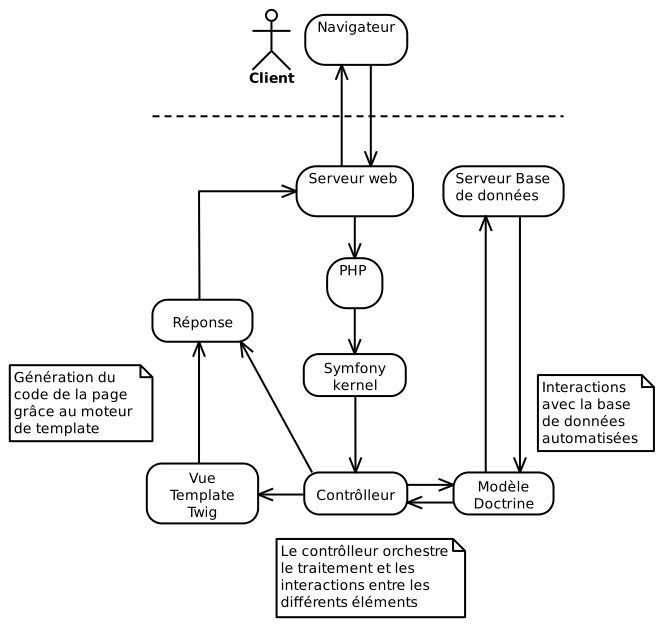
\includegraphics[width=0.7\linewidth]{pictures/mvc.png}
    %\caption{Architecture MVC dans Symfony}
\end{frame}


% structuration
% @Tristan
\section{Structuration}
\sectitle{Structuration des données}

\begin{frame}
    \frametitle{Redondance des événements}
    Le constat :
    \begin{itemize}
        \item Événements redondants
        \item Informations dupliquées
    \end{itemize}
    \pause
    \vspace{2em}
    Notre choix :
    \begin{itemize}
        \item Événements fixes
        \item Nouvelle éditions chaque année
    \end{itemize}
\end{frame}

\begin{frame}
    \frametitle{Inexhaustion des formulaires}
    Le constat :
    \begin{itemize}
        \item Besoins spécifiques par événement
        \item Formulaires souvent similaires
    \end{itemize}
    \pause
    \vspace{2em}
    Notre choix :
    \begin{itemize}
        \item Formulaires personnalisables
        \item Construction récursive
    \end{itemize}
\end{frame}

\begin{frame}
    \frametitle{Gestion de la récurtion}
    Généralisation d'un formulaire $\Longrightarrow$ \textit{\textbf{FormWidget}} \\
    \pause
    \vspace{3em}
    3 types de \textit{FormWidget} :
    \begin{itemize}
        \item<3-> Natif
        \item<4-> Composite
        \item<5-> Liste
    \end{itemize}
\end{frame}

\begin{frame}
    \frametitle{Structure finale de la base de données}
    \begin{figure}
        \centering
        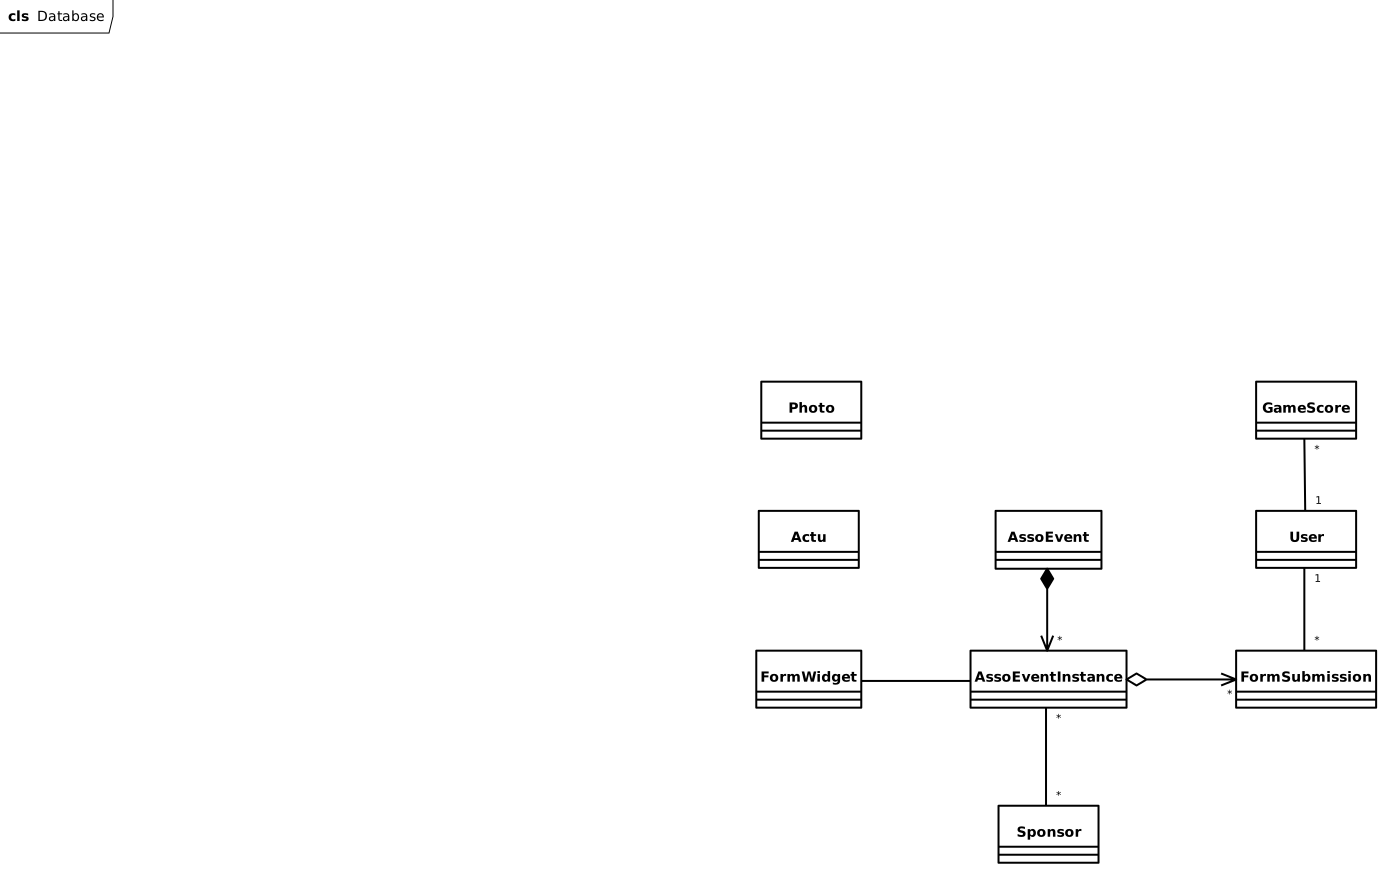
\includegraphics[width=0.8\textwidth]{pictures/database.png}
    \end{figure}
\end{frame}


% démonstration
% @Antoine
\section{Démonstration}
\sectitle{Démonstration du site web}

% conclusion
% @Antoine
\chapter{Bilan}

À l’issue de ce projet, nous avons pu livrer une première version du site de l’OFNI, intégrant les principales fonctionnalités définies en amont. 

Ce développement nous a permis de consolider nos compétences en Symfony, en JavaScript et en Sass, tout en découvrant des outils tels que Figma pour le maquettage et Trello pour la gestion de projet.
\bigskip

Si le site répond globalement aux objectifs fixés, certaines fonctionnalités ont dû être adaptées ou reportées en raison de contraintes techniques ou administratives. Malgré cela, nous avons réussi à implémenter une plateforme complète et évolutive, avec une attention particulière portée à la maintenabilité et à l’expérience utilisateur.
\bigskip

Ce projet nous a également permis de mieux appréhender le travail en équipe sur un projet d’envergure, en nous confrontant à des problématiques concrètes de gestion du temps, de répartition des tâches et d’adaptation aux imprévus. 
\bigskip

Nous espérons que ce site constituera une base solide pour les futurs bureaux de l’OFNI et qu’il pourra être enrichi au fil du temps par de nouvelles améliorations.


\end{document} 
